
The key to resolving our problem is not to attempt to evaluate part of an expression until the whole expression has been seen (in our example, until the assignment operator is invoked). Thus, before the evaluation, we must record which operations are being applied to which objects. The operations are determined at compile time and can therefore be encoded in template arguments.

For our example expression,

\begin{lstlisting}[style=styleCXX]
1.2*x + x*y;
\end{lstlisting}

this means that the result of 1.2*x is not a new array but an object that represents each value of x multiplied by 1.2. Similarly, x*y must yield each element of x multiplied by each corresponding element of y. Finally, when we need the values of the resulting array, we do the computation that we stored for later evaluation.

Let’s design a concrete implementation. Our implementation will evaluate the expression

\begin{lstlisting}[style=styleCXX]
1.2*x + x*y;
\end{lstlisting}

into an object with the following type:

\begin{lstlisting}[style=styleCXX]
A_Add<A_Mult<A_Scalar<double>,Array<double>>,
	  A_Mult<Array<double>,Array<double>>>
\end{lstlisting}

We combine a new fundamental Array class template with class templates A\_Scalar, A\_Add, and A\_Mult. You may recognize a prefix representation for the syntax tree corresponding to this expression (see Figure 27.1). This nested template-id represents the operations involved and the types of the objects to which the operations should be applied. A\_Scalar is presented later but is essentially just a placeholder for a scalar in an array expression.

\begin{center}
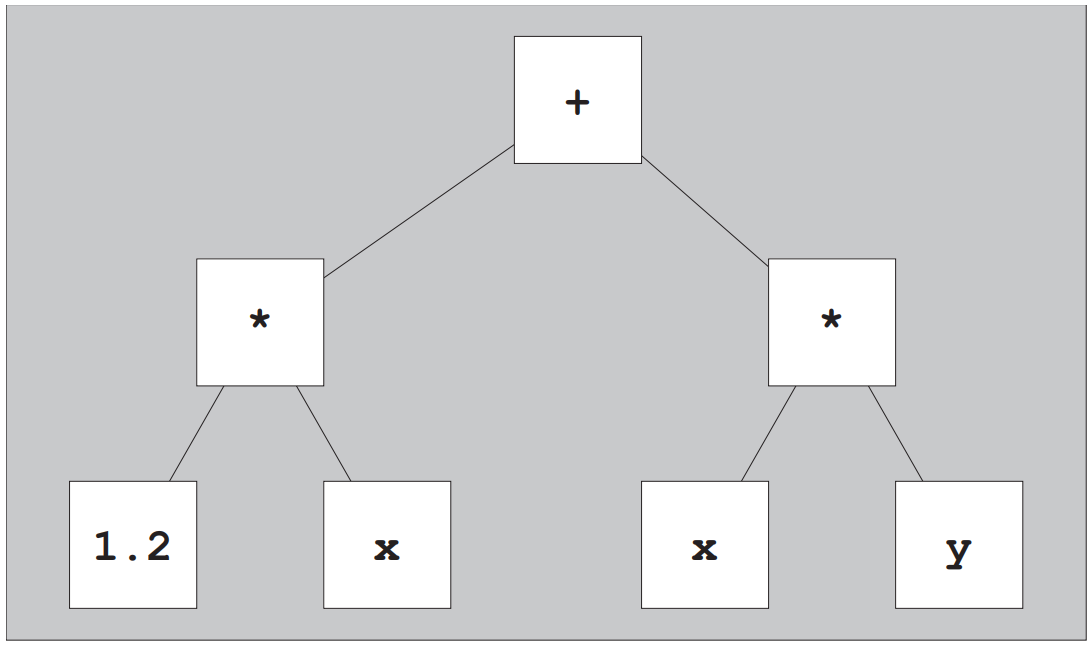
\includegraphics[width=0.8\textwidth]{content/3/chapter27/images/1.png} \\
Figure 27.1. Tree representation of expression 1.2*x+x*y
\end{center}

\subsubsubsection{27.2.1\hspace{0.2cm}Operands of the Expression Templates}

To complete the representation of the expression, we must store references to the arguments in each of the A\_Add and A\_Mult objects and record the value of the scalar in the A\_Scalar object (or a reference thereto). Here are possible definitions for the corresponding operands:

\hspace*{\fill} \\ %插入空行
\noindent
\textit{exprtmpl/exprops1.hpp}
\begin{lstlisting}[style=styleCXX]
#include <cstddef>
#include <cassert>

// include helper class traits template to select whether to refer to an
// expression template node either by value or by reference
#include "exprops1a.hpp"

// class for objects that represent the addition of two operands
template<typename T, typename OP1, typename OP2>
class A_Add {
	private:
	typename A_Traits<OP1>::ExprRef op1; // first operand
	typename A_Traits<OP2>::ExprRef op2; // second operand
	
	public:
	// constructor initializes references to operands
	A_Add (OP1 const& a, OP2 const& b)
	: op1(a), op2(b) {
	}

	// compute sum when value requested
	T operator[] (std::size_t idx) const {
		return op1[idx] + op2[idx];
	}

	// size is maximum size
	std::size_t size() const {
		assert (op1.size()==0 || op2.size()==0
		|| op1.size()==op2.size());
		return op1.size()!=0 ? op1.size() : op2.size();
	}
};

// class for objects that represent the multiplication of two operands
template<typename T, typename OP1, typename OP2>
class A_Mult {
	private:
	typename A_Traits<OP1>::ExprRef op1; // first operand
	typename A_Traits<OP2>::ExprRef op2; // second operand
	
	public:
	// constructor initializes references to operands
	A_Mult (OP1 const& a, OP2 const& b)
	: op1(a), op2(b) {
	}

	// compute product when value requested
	T operator[] (std::size_t idx) const {
		return op1[idx] * op2[idx];
	}

	// size is maximum size
	std::size_t size() const {
		assert (op1.size()==0 || op2.size()==0
		|| op1.size()==op2.size());
		return op1.size()!=0 ? op1.size() : op2.size();
	}
};
\end{lstlisting}

As you can see, we added subscripting and size-querying operations that allow us to compute the size and the values of the elements for the array resulting from the operations represented by the subtree of nodes rooted at the given object.

For operations involving arrays only, the size of the result is the size of either operand. However, for operations involving both an array and a scalar, the size of the result is the size of the array operand. To distinguish array operands from scalar operands, we define a size of zero for scalars. The A\_Scalar template is therefore defined as follows:

\hspace*{\fill} \\ %插入空行
\noindent
\textit{exprtmpl/exprscalar.cpp}
\begin{lstlisting}[style=styleCXX]
// class for objects that represent scalars:
template<typename T>
class A_Scalar {
	private:
	T const& s; // value of the scalar
	
	public:
	// constructor initializes value
	constexpr A_Scalar (T const& v)
	: s(v) {
	}

	// for index operations, the scalar is the value of each element
	constexpr T const& operator[] (std::size_t) const {
		return s;
	}

	// scalars have zero as size
	constexpr std::size_t size() const {
		return 0;
	};
};
\end{lstlisting}

(We have declared the constructor and member functions constexpr so this class can be used at compile time. This is, however, not strictly needed for our purposes.)

Note that scalars also provide an index operator. Inside the expression, they represent an array with the same scalar value for each index.

You probably saw that the operator classes used a helper class A\_Traits to define the members for the operands:

\begin{lstlisting}[style=styleCXX]
typename A_Traits<OP1>::ExprRef op1; // first operand
typename A_Traits<OP2>::ExprRef op2; // second op
\end{lstlisting}

This is necessary because, in general, we can declare them to be references, since most temporary nodes are bound in the top-level expression and therefore live until the end of the evaluation of that complete expression. The one exception are the A\_Scalar nodes. They are bound within the operator functions and might not live until the end of the evaluation of the complete expression. Thus, to avoid having members refer to scalars that no longer exist, the A\_Scalar operands have to be copied by value.

In other words, we need members that are

\begin{itemize}
\item 
constant references in general:
\begin{lstlisting}[style=styleCXX]
OP1 const& op1; // refer to first operand by reference
OP2 const& op2; // refer to second operand by reference
\end{lstlisting}

\item 
but ordinary values for scalars:
\begin{lstlisting}[style=styleCXX]
OP1 op1; // refer to first operand by value
OP2 op2; // refer to second operand by value
\end{lstlisting}
\end{itemize}

This is a perfect application of traits classes. The traits class defines a type to be a constant reference in general but an ordinary value for scalars:

\hspace*{\fill} \\ %插入空行
\noindent
\textit{exprtmpl/exprops1a.hpp}
\begin{lstlisting}[style=styleCXX]
// helper traits class to select how to refer to an expression template node
// - in general by reference
// - for scalars by value

template<typename T> class A_Scalar;

// primary template
template<typename T>
class A_Traits {
	public:
	using ExprRef = T const&; // type to refer to is constant reference
};

// partial specialization for scalars
template<typename T>
class A_Traits<A_Scalar<T>> {
	public:
	using ExprRef = A_Scalar<T>; // type to refer to is ordinary value
};
\end{lstlisting}

Note that since A\_Scalar objects refer to scalars in the top-level expression, those scalars can use reference types. That is, A\_Scalar<T>::s is a reference member.

\subsubsubsection{27.2.2\hspace{0.2cm}The ArrayType}

With our ability to encode expressions using lightweight expression templates, we must now create an Array type that controls actual storage and that knows about the expression templates. However, it is also useful for engineering purposes to keep as similar as possible the interface for a real array with storage and one for a representation of an expression that results in an array. To this end, we declare the Array template as follows:

\begin{lstlisting}[style=styleCXX]
template<typename T, typename Rep = SArray<T>>
class Array;
\end{lstlisting}

The type Rep can be SArray if Array is a real array of storage,

\begin{tcolorbox}[colback=webgreen!5!white,colframe=webgreen!75!black]
\hspace*{0.75cm}It is convenient to reuse the previously developed SArray here, but in an industrial-strength library, a specialpurpose implementation may be preferable because we won’t use all the features of SArray.
\end{tcolorbox}

or it can be the nested template-id such as A\_Add or A\_Mult that encodes an expression. Either way we are handling Array instantiations, which considerably simplify our later dealings. In fact, even the definition of the Array template needs no specializations to distinguish the two cases, although some of the members cannot be instantiated for types like A\_Mult substituted for Rep.

Here is the definition. The functionality is limited roughly to what was provided by our SArray template, although once the code is understood, it is not hard to add to that functionality:

\hspace*{\fill} \\ %插入空行
\noindent
\textit{exprtmpl/exprarray.hpp}
\begin{lstlisting}[style=styleCXX]
#include <cstddef>
#include <cassert>
#include "sarray1.hpp"

template<typename T, typename Rep = SArray<T>>
class Array {
	private:
	Rep expr_rep; // (access to) the data of the array
	
	public:
	// create array with initial size
	explicit Array (std::size_t s)
	: expr_rep(s) {
	}

	// create array from possible representation
	Array (Rep const& rb)
	: expr_rep(rb) {
	}

	// assignment operator for same type
	Array& operator= (Array const& b) {
		assert(size()==b.size());
		for (std::size_t idx = 0; idx<b.size(); ++idx) {
			expr_rep[idx] = b[idx];
		}
		return *this;
	}

	// assignment operator for arrays of different type
	template<typename T2, typename Rep2>
	Array& operator= (Array<T2, Rep2> const& b) {
		assert(size()==b.size());
		for (std::size_t idx = 0; idx<b.size(); ++idx) {
			expr_rep[idx] = b[idx];
		}
		return *this;
	}

	// size is size of represented data
	std::size_t size() const {
		return expr_rep.size();
	}

	// index operator for constants and variables
	decltype(auto) operator[] (std::size_t idx) const {
		assert(idx<size());
		return expr_rep[idx];
	}
	T& operator[] (std::size_t idx) {
		assert(idx<size());
		return expr_rep[idx];
	}

	// return what the array currently represents
	Rep const& rep() const {
		return expr_rep;
	}
	Rep& rep() {
		return expr_rep;
	}
};
\end{lstlisting}

As you can see, many operations are simply forwarded to the underlying Rep object. However, when copying another array, we must take into account the possibility that the other array is really built on an expression template. Thus, we parameterize these copy operations in terms of the underlying Rep representation.

The subscripting operator deserves a little discussion. Note that the const version of that operator uses a deduced return type rather than the more traditional type T const\&. We do that because if Rep represents is A\_Mult or A\_Add, its subscripting operator returns a temporary value (i.e., a prvalue), which cannot be returned by reference (and decltype(auto) will deduce a nonreference type for the prvalue case). On the other hand, if Rep is SArray<T> then the underlying subscript operator produces a const lvalue, and the deduced return type will be a matching const reference for that case.

\subsubsubsection{27.2.3\hspace{0.2cm}The Operators}

We have most of the machinery in place to have efficient numeric operators for our numeric Array template, except the operators themselves. As implied earlier, these operators only assemble the expression template objects—they don’t actually evaluate the resulting arrays.

For each ordinary binary operator, we must implement three versions: array-array, array-scalar, and scalar-array. To be able to compute our initial value, we need, for example, the following operators:

\hspace*{\fill} \\ %插入空行
\noindent
\textit{exprtmpl/exprops2.hpp}
\begin{lstlisting}[style=styleCXX]
// addition of two Arrays:
template<typename T, typename R1, typename R2>
Array<T,A_Add<T,R1,R2>>
operator+ (Array<T,R1> const& a, Array<T,R2> const& b) {
	return Array<T,A_Add<T,R1,R2>>
		(A_Add<T,R1,R2>(a.rep(),b.rep()));
}

// multiplication of two Arrays:
template<typename T, typename R1, typename R2>
Array<T, A_Mult<T,R1,R2>>
operator* (Array<T,R1> const& a, Array<T,R2> const& b) {
	return Array<T,A_Mult<T,R1,R2>>
		(A_Mult<T,R1,R2>(a.rep(), b.rep()));
}

// multiplication of scalar and Array:
template<typename T, typename R2>
Array<T, A_Mult<T,A_Scalar<T>,R2>>
operator* (T const& s, Array<T,R2> const& b) {
	return Array<T,A_Mult<T,A_Scalar<T>,R2>>
		(A_Mult<T,A_Scalar<T>,R2>(A_Scalar<T>(s), b.rep()));
}

// multiplication of Array and scalar, addition of scalar and Array
// addition of Array and scalar:
...
\end{lstlisting}

The declaration of these operators is somewhat cumbersome (as can be seen from these examples), but the functions really don’t do much. For example, the plus operator for two arrays first creates an A\_Add<> object that represents the operator and the operands

\begin{lstlisting}[style=styleCXX]
A_Add<T,R1,R2>(a.rep(),b.rep())
\end{lstlisting}

and wraps this object in an Array object so that we can use the result as any other object that represents data of an array:

\begin{lstlisting}[style=styleCXX]
return Array<T,A_Add<T,R1,R2>> (...);
\end{lstlisting}

For scalar multiplication, we use the A\_Scalar template to create the A\_Mult object

\begin{lstlisting}[style=styleCXX]
A_Mult<T,A_Scalar<T>,R2>(A_Scalar<T>(s), b.rep())
\end{lstlisting}

and wrap again:

\begin{lstlisting}[style=styleCXX]
return Array<T,A_Mult<T,A_Scalar<T>,R2>> (...);
\end{lstlisting}

Other nonmember binary operators are so similar that macros can be used to cover most operators with relatively little source code. Another (smaller) macro could be used for nonmember unary operators.

\subsubsubsection{27.2.4\hspace{0.2cm}Review}

On first discovery of the expression template idea, the interaction of the various declarations and definitions can be daunting. Hence, a top-down review of what happens with our example code may help crystallize understanding. The code we will analyze is the following (you can find it as part of meta/exprmain.cpp):

\begin{lstlisting}[style=styleCXX]
int main()
{
	Array<double> x(1000), y(1000);
	...
	x = 1.2*x + x*y;
}
\end{lstlisting}

Because the Rep argument is omitted in the definition of x and y, it is set to the default, which is SArray<double>. So, x and y are arrays with “real” storage and not just recordings of operations.

When parsing the expression

\begin{lstlisting}[style=styleCXX]
1.2*x + x*y
\end{lstlisting}

the compiler first applies the leftmost * operation, which is a scalar-array operator. Overload resolution thus selects the scalar-array form of operator*:

\begin{lstlisting}[style=styleCXX]
template<typename T, typename R2>
Array<T, A_Mult<T,A_Scalar<T>,R2>>
operator* (T const& s, Array<T,R2> const& b) {
	return Array<T,A_Mult<T,A_Scalar<T>,R2>>
		(A_Mult<T,A_Scalar<T>,R2>(A_Scalar<T>(s), b.rep()));
}
\end{lstlisting}

The operand types are double and Array<double, SArray<double>>. Thus, the type of the result is

\begin{lstlisting}[style=styleCXX]
Array<double, A_Mult<double, A_Scalar<double>, SArray<double>>>
\end{lstlisting}

The result value is constructed to reference an A\_Scalar<double> object constructed from the double value 1.2 and the SArray<double> representation of the object x.

Next, the second multiplication is evaluated: It is an array-array operation x*y. This time we use the appropriate operator*:

\begin{lstlisting}[style=styleCXX]
template<typename T, typename R1, typename R2>
Array<T, A_Mult<T,R1,R2>>
operator* (Array<T,R1> const& a, Array<T,R2> const& b) {
	return Array<T,A_Mult<T,R1,R2>>
		(A_Mult<T,R1,R2>(a.rep(), b.rep()));
}
\end{lstlisting}

The operand types are both Array<double, SArray<double>>, so the result type is

\begin{lstlisting}[style=styleCXX]
Array<double, A_Mult<double, SArray<double>, SArray<double>>>
\end{lstlisting}

This time the wrapped A\_Mult object refers to two SArray<double> representations: the one of x and the one of y.

Finally, the + operation is evaluated. It is again an array-array operation, and the operand types are the result types that we just deduced. So, we invoke the array-array operator +:

\begin{lstlisting}[style=styleCXX]
template<typename T, typename R1, typename R2>
Array<T,A_Add<T,R1,R2>>
operator+ (Array<T,R1> const& a, Array<T,R2> const& b) {
	return Array<T,A_Add<T,R1,R2>>
		(A_Add<T,R1,R2>(a.rep(),b.rep()));
}
\end{lstlisting}

T is substituted with double, whereas R1 is substituted with

\begin{lstlisting}[style=styleCXX]
A_Mult<double, A_Scalar<double>, SArray<double>>
\end{lstlisting}

and R2 is substituted with

\begin{lstlisting}[style=styleCXX]
A_Mult<double, SArray<double>, SArray<double>>
\end{lstlisting}

Hence, the type of the expression to the right of the assignment token is

\begin{lstlisting}[style=styleCXX]
Array<double,
	A_Add<double,
		A_Mult<double, A_Scalar<double>, SArray<double>>,
		A_Mult<double, SArray<double>, SArray<double>>>>
\end{lstlisting}

This type is matched to the assignment operator template of the Array template:

\begin{lstlisting}[style=styleCXX]
template<typename T, typename Rep = SArray<T>>
class Array {
	public:
	...
	// assignment operator for arrays of different type
	template<typename T2, typename Rep2>
	Array& operator= (Array<T2, Rep2> const& b) {
		assert(size()==b.size());
		for (std::size_t idx = 0; idx<b.size(); ++idx) {
			expr_rep[idx] = b[idx];
		}
		return *this;
	}
...
};
\end{lstlisting}

The assignment operator computes each element of the destination x by applying the subscript operator to the representation of the right side, the type of which is

\begin{lstlisting}[style=styleCXX]
A_Add<double,
	A_Mult<double, A_Scalar<double>, SArray<double>>,
	A_Mult<double, SArray<double>, SArray<double>>>>
\end{lstlisting}

Carefully tracing this subscript operator shows that for a given subscript idx, it computes

\begin{lstlisting}[style=styleCXX]
(1.2*x[idx]) + (x[idx]*y[idx])
\end{lstlisting}

which is exactly what we want.

\subsubsubsection{27.2.5\hspace{0.2cm}Expression Templates Assignments}

It is not possible to instantiate write operations for an array with a Rep argument that is built on our example A\_Mult and A\_Add expression templates. (Indeed, it makes no sense to write a+b = c.) However, it is entirely reasonable to write other expression templates for which assignment to the result is possible. For example, indexing with an array of integral values would intuitively correspond to subset selection. In other words, the expression

\begin{lstlisting}[style=styleCXX]
x[y] = 2*x[y];
\end{lstlisting}

should mean the same as

\begin{lstlisting}[style=styleCXX]
for (std::size_t idx = 0; idx<y.size(); ++idx) {
	x[y[idx]] = 2*x[y[idx]];
}
\end{lstlisting}

Enabling this implies that an array built on an expression template behaves like an lvalue (i.e., is writable). The expression template component for this is not fundamentally different from, say, A\_Mult, except that both const and non-const versions of the subscript operators are provided, and they may return lvalues (references):

\hspace*{\fill} \\ %插入空行
\noindent
\textit{exprtmpl/exprops3.hpp}
\begin{lstlisting}[style=styleCXX]
template<typename T, typename A1, typename A2>
class A_Subscript {
	public:
	// constructor initializes references to operands
	A_Subscript (A1 const& a, A2 const& b)
	: a1(a), a2(b) {
	}

	// process subscription when value requested
	decltype(auto) operator[] (std::size_t idx) const {
		return a1[a2[idx]];
	}
	T& operator[] (std::size_t idx) {
		return a1[a2[idx]];
	}

	// size is size of inner array
	std::size_t size() const {
		return a2.size();
	}
	private:
	A1 const& a1; // reference to first operand
	A2 const& a2; // reference to second operand
};
\end{lstlisting}

Again, decltype(auto) comes in handy to handle subscripting of arrays independently of whether the underlying representation produces prvalues or lvalues.

The extended subscript operator with subset semantics that was suggested earlier would require that additional subscript operators be added to the Array template. One of these operators could be defined as follows (a corresponding const version would presumably also be needed):

\hspace*{\fill} \\ %插入空行
\noindent
\textit{exprtmpl/exprops4.hpp}
\begin{lstlisting}[style=styleCXX]
template<typename T, typename R>
template<typename T2, typename R2>
Array<T, A_Subscript<T, R, R2>>
Array<T, R>::operator[](Array<T2, R2> const& b) {
	return Array<T, A_Subscript<T, R, R2>>
		(A_Subscript<T, R, R2>(*this, b));
}
\end{lstlisting}













